% !TEX program = pdflatex
\documentclass[9pt]{extarticle}
\usepackage[letterpaper,margin=0.58in,top=0.64in,bottom=0.58in]{geometry}
\usepackage[T1]{fontenc}
\usepackage{lmodern}
\usepackage{graphicx}
\usepackage{booktabs}
\usepackage{tabularx}
\usepackage{array}
\usepackage{xcolor}
\usepackage{fancyhdr}
\usepackage{titlesec}
\usepackage{enumitem}
\usepackage{hyperref}
\usepackage{microtype}
\usepackage{ragged2e}

\definecolor{navy}{HTML}{193946}
\definecolor{teal}{HTML}{0A7C74}
\definecolor{lightteal}{HTML}{E8F2F1}
\definecolor{amber}{HTML}{D67A35}
\definecolor{lightamber}{HTML}{FFF4E8}
\definecolor{red}{HTML}{B94A48}
\definecolor{lightred}{HTML}{FCEEEE}
\definecolor{slate}{HTML}{526C75}
\definecolor{rulegray}{HTML}{C9D7DA}
\definecolor{lightblue}{HTML}{EEF4F7}

\hypersetup{colorlinks=true,urlcolor=teal,linkcolor=teal}
\pagestyle{fancy}
\fancyhf{}
\lhead{\textcolor{slate}{ECG feature-matrix audit}}
\rhead{\textcolor{slate}{PI briefing}}
\cfoot{\textcolor{slate}{\thepage\ / 4}}
\renewcommand{\headrulewidth}{0.35pt}
\setlength{\headheight}{12pt}
\setlength{\parindent}{0pt}
\setlength{\parskip}{3pt}
\setlist[itemize]{leftmargin=1.2em,itemsep=1.6pt,topsep=2pt}
\setlist[enumerate]{leftmargin=1.4em,itemsep=1.8pt,topsep=2pt}
\titleformat{\section}{\large\bfseries\color{navy}}{}{0pt}{}
\titlespacing*{\section}{0pt}{5pt}{3pt}
\newcolumntype{Y}{>{\RaggedRight\arraybackslash}X}
\newcolumntype{L}[1]{>{\RaggedRight\arraybackslash}p{#1}}
\newcolumntype{C}[1]{>{\centering\arraybackslash}p{#1}}
\newcolumntype{R}[1]{>{\raggedleft\arraybackslash}p{#1}}

\newcommand{\pageheading}[2]{%
  {\fontsize{18}{20}\selectfont\bfseries\color{navy} #1}\par
  {\small\color{slate} #2}\par\vspace{3pt}\color{rulegray}\hrule\color{black}\vspace{5pt}
}
\newcommand{\conclusion}[1]{%
  \noindent\fcolorbox{teal}{lightteal}{\parbox{0.965\linewidth}{\textbf{Clear conclusion.} #1}}\par
}
\newcommand{\warningbox}[1]{%
  \noindent\fcolorbox{amber}{lightamber}{\parbox{0.965\linewidth}{\textbf{Do not over-interpret this.} #1}}\par
}
\newcommand{\nextbox}[1]{%
  \noindent\fcolorbox{navy}{lightblue}{\parbox{0.965\linewidth}{\textbf{What this means for the next step.} #1}}\par
}

\begin{document}

% -----------------------------------------------------------------------------
% PAGE 1
% -----------------------------------------------------------------------------
\pageheading{What the extracted ECG feature matrix can and cannot do}{A four-page, seizure-focused interpretation for discussion with the PI}

\conclusion{The 52 extracted features describe signal quality well and contain useful abnormal-beat information. They do \emph{not} yet provide a reliable seizure detector. The seizure limitation is a combination of too few independent patients and a feature design centred on individual beats rather than changes over time.}

\begin{center}
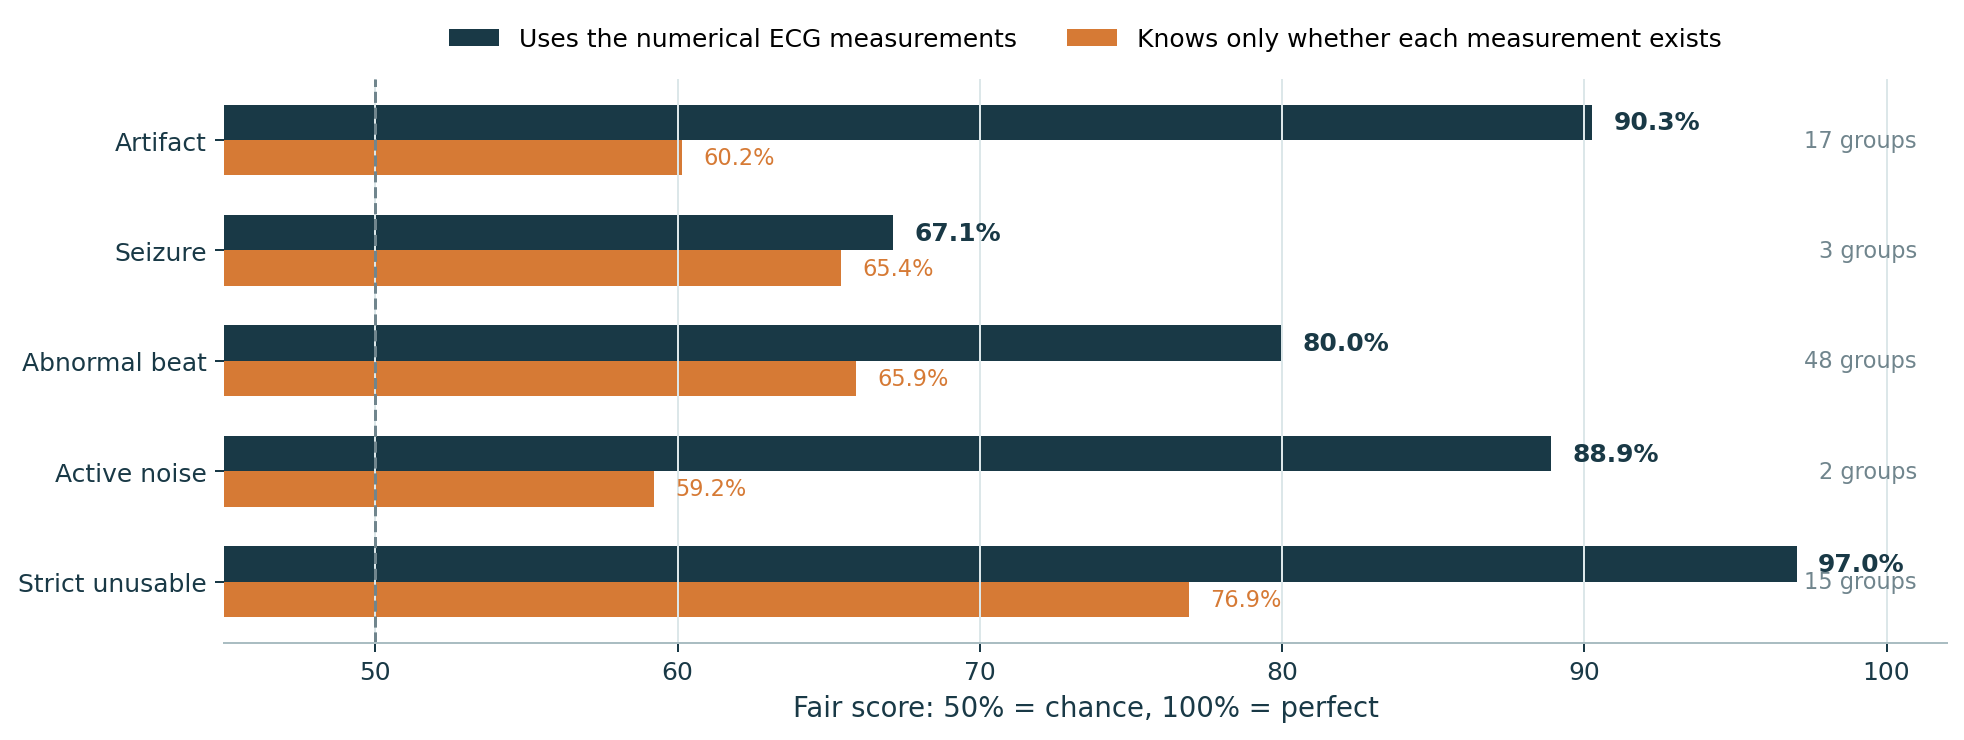
\includegraphics[width=0.99\linewidth]{simple_overview.png}
\end{center}
\vspace{-6pt}

\begin{tabularx}{\linewidth}{@{}L{1.02in}C{0.52in}C{0.46in}C{0.46in}C{0.46in}C{0.52in}C{0.40in}Y@{}}
\toprule
Target & Fair score* & Found & Ignored & Alerts right & AUC & Groups & Plain conclusion \\
\midrule
Artifact & 90.3\% & 87.9\% & 93.7\% & 94.5\% & 95.4\% & 17 & Strong internal result \\
Seizure & 67.1\% & 63.0\% & 71.0\% & 19.7\% & 73.1\% & 3 & Weak; too many false alerts \\
Abnormal beat & 80.0\% & 69.9\% & 90.2\% & 64.3\% & 90.1\% & 48 & Moderate; varies by patient \\
Active noise & 88.9\% & 82.2\% & 95.7\% & 97.9\% & 95.0\% & 2 & Strong-looking; not generalizable yet \\
Strict unusable & 97.0\% & 92.7\% & 98.0\% & 88.0\% & 98.4\% & 15 & Strong, but a narrow quality task \\
\bottomrule
\end{tabularx}

\section*{What every statistic means in ordinary language}
\begin{tabularx}{\linewidth}{@{}L{1.28in}Y L{2.25in}@{}}
\toprule
Report term & Ask this clinical question & How to interpret it \\
\midrule
Fair score* (group BA) & Does the model handle both positive and negative cases fairly? & Average of ``found'' and ``ignored.'' 50\% is coin-flip performance. Each patient/source receives equal weight, so one long recording cannot dominate. \\
Found (sensitivity) & Out of 100 real seizures/artifacts, how many did it find? & Seizure: 63 found and 37 missed. \\
Ignored (specificity) & Out of 100 non-seizure/non-artifact cases, how many did it correctly leave alone? & Seizure: 71 ignored and 29 falsely flagged. \\
Alerts right (PPV) & Out of 100 alarms, how many were genuine? & Seizure: only about 20 genuine; about 80 false. \\
AUC & Does a genuine case usually receive a higher risk score than a non-case? & 50\% is random ranking; 100\% is perfect ranking. It is \emph{not} the percentage of correct alarms. \\
\bottomrule
\end{tabularx}

\warningbox{The navy and orange bars are two separate tests. Navy uses the numerical ECG measurements. Orange is deliberately denied those numbers and is told only whether each measurement exists. Page 2 gives a concrete example.}

\vfill
{\scriptsize\color{slate}\textbf{Audit scope:} 39,664 rows, 52 model features, 56 label/provenance fields, 266 lineage groups and 375 model/feature-branch tests. An independent rebuild reproduced every feature value and label exactly.}

\newpage

% -----------------------------------------------------------------------------
% PAGE 2
% -----------------------------------------------------------------------------
\pageheading{Seizure is the clear weakness}{The numerical measurements barely improve on knowing only whether measurements were available}

\begingroup
\small
\renewcommand{\arraystretch}{0.92}

\begin{center}
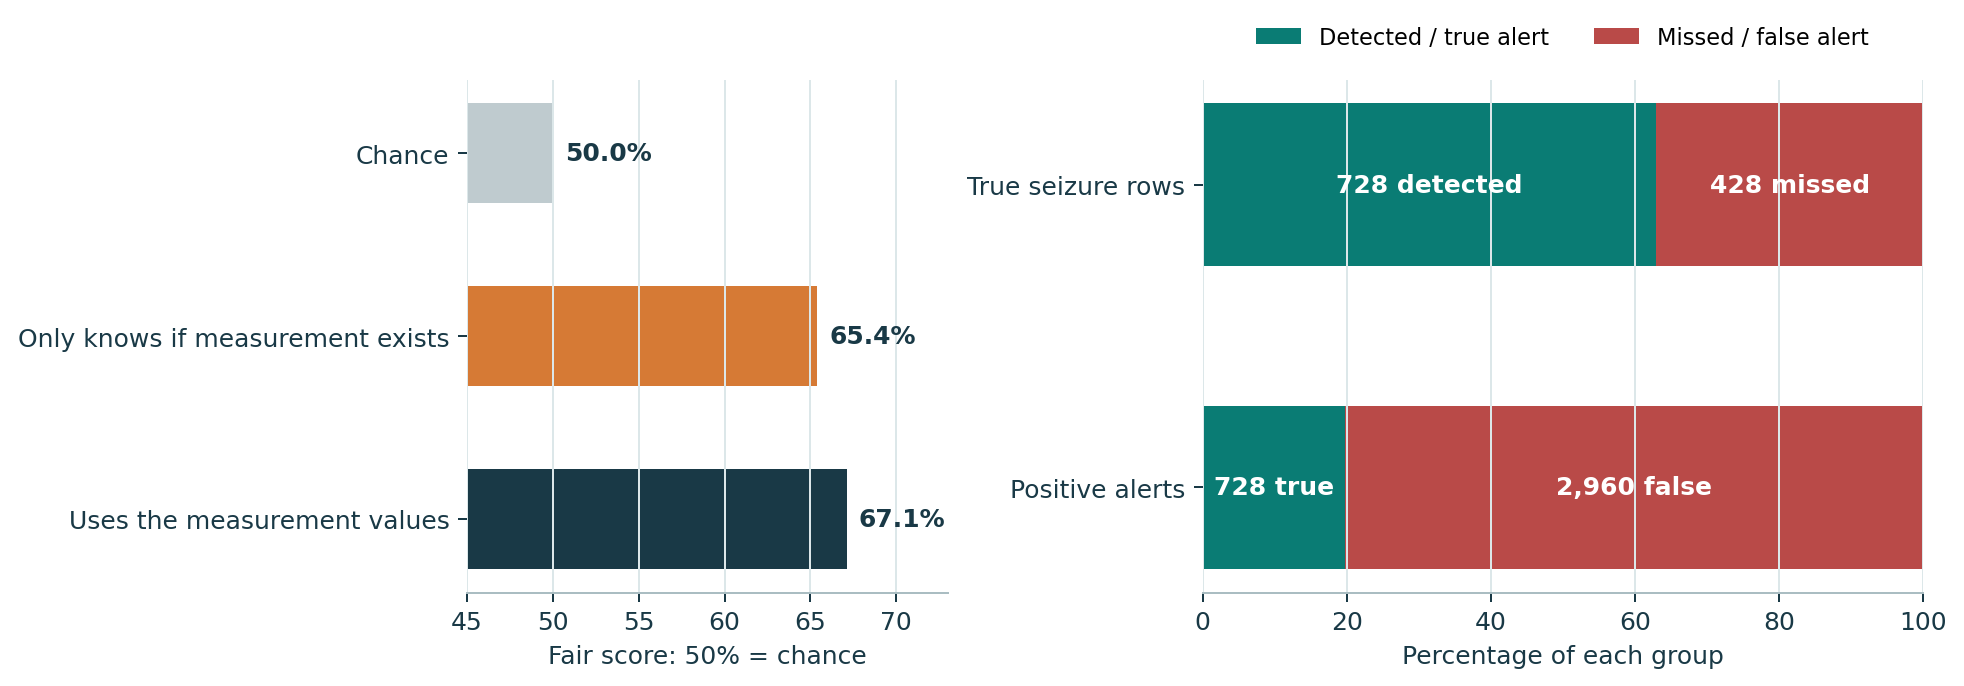
\includegraphics[width=0.88\linewidth]{seizure_reality.png}
\end{center}
\vspace{-8pt}

\conclusion{For seizure, the numerical ECG measurements achieved a 67.1\% patient-weighted fair score. A control told only whether each measurement existed achieved 65.4\%. The improvement is only 1.7 percentage points, so the current matrix has not learned a strong seizure signature.}

\section*{Exactly how to read the seizure row}
\begin{tabularx}{\linewidth}{@{}L{1.05in}Y@{}}
\toprule
Number shown & What it means for these seizure predictions \\
\midrule
67.1\% fair score & Overall ability to separate seizure from non-seizure while giving both sides equal importance. It is better than the 50\% chance level, but not strong. \\
63.0\% found & Of 1,156 true seizure rows, 728 were detected and 428 were missed. \\
71.0\% ignored & Of 10,190 non-seizure rows, 7,230 were correctly left alone and 2,960 were falsely flagged. \\
19.7\% alerts right & The model produced 3,688 seizure alerts, but only 728 were correct. About four out of every five alerts were false. \\
73.1\% AUC & Seizure rows often received somewhat higher scores than non-seizure rows when every possible alarm cutoff was considered. It does \emph{not} mean 73.1\% of alarms were correct. \\
3 independent groups & The nine recording files come from only three independent patient/source groups. Nine files do not equal nine independent patients. \\
\bottomrule
\end{tabularx}

\warningbox{Nothing in the seizure row is 90\%. The 90.3\% fair score belongs to artifact detection, not seizure detection.}

\section*{Feature availability versus an actual ECG feature}
\begin{tabularx}{\linewidth}{@{}L{1.22in}L{2.30in}Y@{}}
\toprule
Example & Availability-only test sees & Actual-feature test sees \\
\midrule
Heart rate & ``Was it calculated? Yes.'' & ``The heart rate is 112 beats/min.'' \\
RR variability & ``Was it calculated? Yes.'' & ``The variability is 38 ms.'' \\
QRS width & ``Was it calculated? No.'' & No numerical measurement is available. \\
\bottomrule
\end{tabularx}

The availability test sees only a pattern such as \textbf{yes, yes, no}; it never sees 112 beats/min or 38 ms. It can still make guesses from dataset-specific missing-value patterns. The actual-feature test sees the numerical measurements extracted from the ECG, but not the raw waveform.

\section*{Why this remains a weak seizure result}
There were too many false alarms, only three independent groups, and the matrix mainly describes isolated beats. Seizure effects are more likely to appear as sustained changes in heart rate, beat-to-beat variability and ECG shape relative to the patient's baseline before, during and after an episode.

\section*{Concrete weak case: PN06\_5}
For record PN06\_5, the model detected only 22 of 71 seizure rows and missed 49. It also alerted on 327 non-seizure rows. Its fair score was 49.3\%, and only 6.3\% of its alerts were correct: essentially chance performance for this record.

\nextbox{This does not mean ECG can never help detect seizures. It means this sample and beat-centred design are insufficient. Add more independent seizure patients, then describe changes over time relative to each patient's usual ECG and evaluate whole seizure episodes.}

\endgroup

\newpage

% -----------------------------------------------------------------------------
% PAGE 3
% -----------------------------------------------------------------------------
\pageheading{Where the matrix fails under harder conditions}{Abnormal morphology and noise reduce one another's sensitivity; strong averages also contain weak records}

\begin{center}
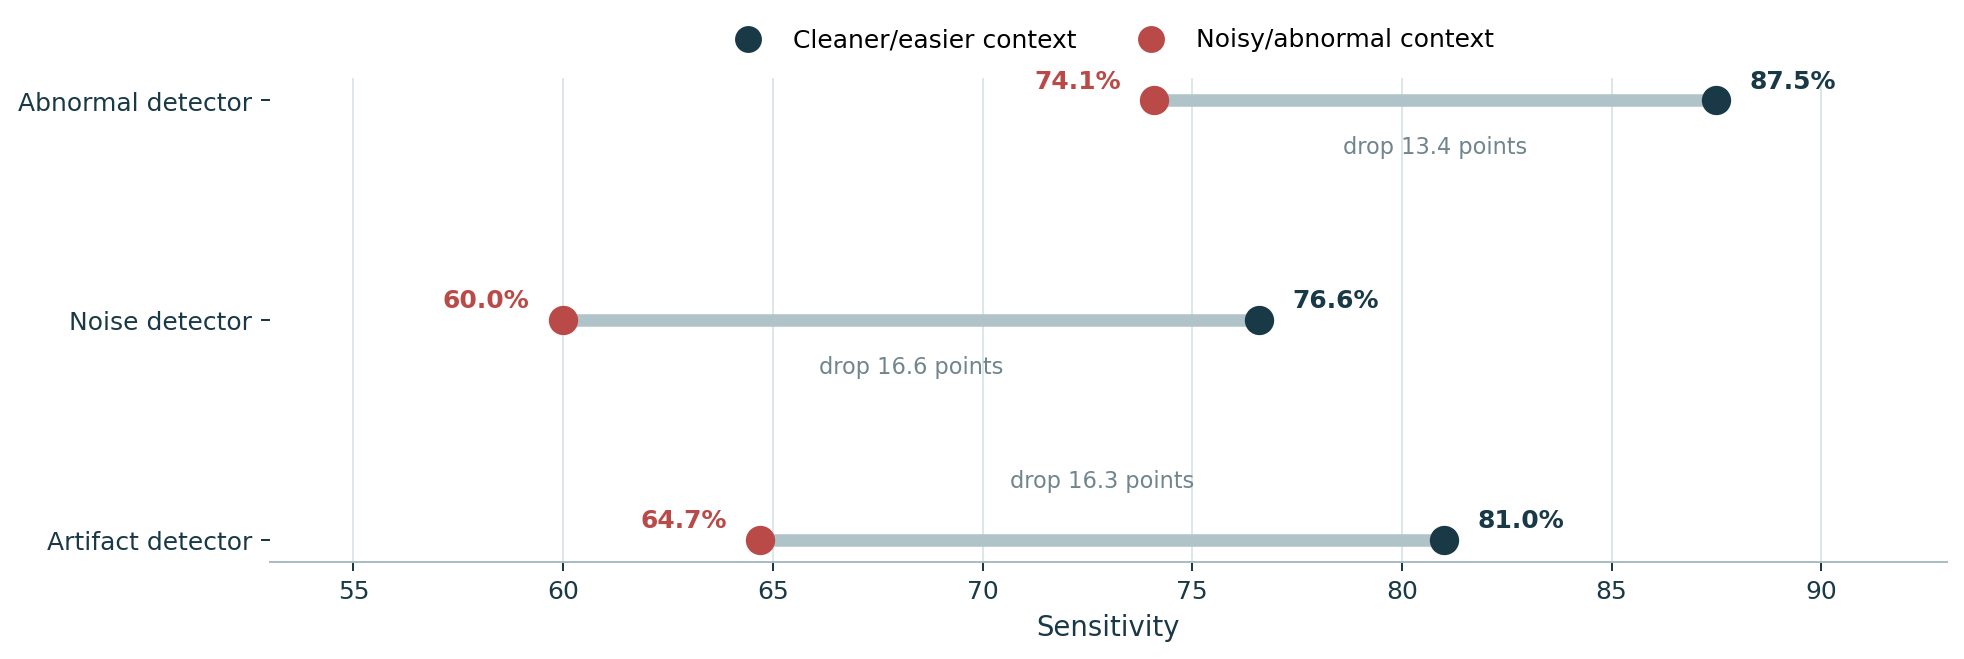
\includegraphics[width=0.98\linewidth]{mixed_context_simple.png}
\end{center}
\vspace{-6pt}

\conclusion{When abnormal beats and noise coexist, detection becomes harder in both directions. Abnormal-beat sensitivity falls by 13.4 points during noise; noise sensitivity falls by 16.6 points on abnormal beats; artifact sensitivity falls by 16.3 points on abnormal beats.}

\section*{How consistent was performance between patient/source groups?}
\begin{tabularx}{\linewidth}{@{}L{1.06in}C{0.65in}C{0.76in}C{0.70in}C{0.70in}Y@{}}
\toprule
Target & Mixed groups & Typical fair score & Middle half & Worst group & Interpretation \\
\midrule
Artifact & 15 & 95.0\% & 85.2--96.6\% & 63.0\% & Usually strong; one important low group \\
Seizure & 3 & 67.4\% & 66.3--68.1\% & 65.2\% & Consistently weak; none reached 80\% \\
Abnormal beat & 40 & 82.3\% & 70.3--96.1\% & 49.5\% & Broad evidence but large variation; six below 60\% \\
Active noise & 2 & 88.9\% & 88.7--89.1\% & 88.6\% & Too few independent groups \\
Strict unusable & 7 & 99.9\% & 99.5--100\% & 87.2\% & Strong in seven mixed groups; eight others had one class \\
\bottomrule
\end{tabularx}

\section*{Weak records that the average hides}
\begin{tabularx}{\linewidth}{@{}L{1.43in}C{0.65in}C{0.65in}Y@{}}
\toprule
Task and record & Cases found & Fair score & What failed \\
\midrule
Artifact: NSTDB 118e24 & 26.1\% & 60.4\% & 116 of 157 artifact rows were missed despite high overall artifact performance. \\
Active noise: NSTDB 118e24 & 42.0\% & 63.8\% & 91 of 157 noisy rows were missed. \\
Abnormal beat: MIT-BIH 207 & 35.0\% & Not defined & 67 of 103 abnormal anchors were missed; this selected window had no negatives. \\
Strict unusable: BUT 111001 & 74.5\% & 87.2\% & 47 of 184 unusable rows were missed even though there were no false unusable alarms. \\
\bottomrule
\end{tabularx}

\section*{What combinations could not be tested?}
Noise/artifact and beat type coexist in 2,158 NSTDB rows, so the comparisons above are valid. The seizure records do not have synchronized noise schedules, expert AAMI beat classes or BUT-QDB quality labels. Therefore seizure plus noise, seizure plus abnormal beat and seizure plus artifact are \textbf{not evaluable} in this matrix. Unknown labels were excluded, not changed to zero.

\warningbox{A high average can hide false reassurance for one patient. The next model should be judged by patient-level distributions, the weakest groups and mixed-condition sensitivity, not only its overall average.}

\vfill
{\scriptsize\color{slate}\textbf{Quality-label detail:} artifact combines degraded and unusable quality with active NSTDB noise. The strict unusable task is narrower: pure BUT-QDB class 1 versus class 3, with the intermediate class deliberately excluded.}

\newpage

% -----------------------------------------------------------------------------
% PAGE 4
% -----------------------------------------------------------------------------
\pageheading{What should change next}{A seizure-specific data and feature redesign, followed by a locked patient-level test}

\begin{tabularx}{\linewidth}{@{}C{0.37in}L{1.30in}L{2.18in}Y@{}}
\toprule
Step & Evidence requiring action & Change & How to know it helped \\
\midrule
1 & Only three seizure groups & Add substantially more independent seizure patients, seizure episodes and difficult non-seizure controls. & Performance remains stable for entirely unseen patients and sources. \\
2 & Rhythm and beat-to-beat timing performed best & Build 30-second, 1-minute, 2-minute and 5-minute summaries: heart-rate acceleration, changing beat-to-beat variability, rhythm irregularity, abnormal-beat burden, ECG-shape trends and change from the patient's usual level. & The new over-time features beat the current features when tested on exactly the same unseen patients. \\
3 & The yes/no availability test already scored 65.4\% & Use the same measurement panel across datasets; rerun without the yes/no availability clues; test rows with a complete common panel and test on an entirely different dataset. & Numerical ECG values clearly beat the yes/no control for each held-out patient, not just on average. \\
4 & Individual-row alerts produced 2,960 false alarms & Judge whole seizure episodes; require a pattern to persist; choose the alarm cutoff carefully; allow ``uncertain'' when signal quality is poor. & More seizure episodes found, fewer false alarms per hour and acceptable time to detection. \\
5 & The winner was chosen from 375 tested options & Make every model and feature choice using training patients only. Then lock the complete method before one final test on untouched external patients. & The locked method repeats its performance in a new patient group, device and clinical-site mix. \\
\bottomrule
\end{tabularx}

\section*{The next experiment I would run}
\begin{enumerate}
\item Keep the current best seizure model---rhythm/beat-timing features with a linear SVM---as the fixed baseline. Do not tune it again using the final test patients.
\item Build three versions: \textbf{A} current features; \textbf{B} the same measurements available across every dataset; and \textbf{C} new features describing changes across 30 seconds to 5 minutes relative to each patient's usual level.
\item Compare A, B and C on exactly the same held-out patients. Choose the model, features and alarm cutoff using training patients only.
\item Report the percentage of seizure episodes found, false alarms per hour, time to detection, percentage of alarms correct, fair score for each patient and improvement over the yes/no availability control.
\item Keep PN06\_5 and the other weak records as fixed challenge cases. Improvement is credible only if the weakest patients improve, not merely the average.
\end{enumerate}

\section*{Recommended cascade}
\noindent\fcolorbox{navy}{lightblue}{\parbox{0.965\linewidth}{\centering
\textbf{Raw ECG} $\longrightarrow$ \textbf{quality and uncertainty} $\longrightarrow$ \textbf{beat detection} $\longrightarrow$ \textbf{temporal seizure features} $\longrightarrow$ \textbf{episode score} $\longrightarrow$ \textbf{alert / no alert / uncertain}
}}

\section*{What can be said to the PI now}
\begin{minipage}[t]{0.48\linewidth}
\textbf{Supported by this audit}
\begin{itemize}
\item The matrix was rebuilt exactly and evaluated without patient/source overlap.
\item The features are useful for signal quality and contain moderate abnormal-beat information.
\item The present seizure representation is inadequate and its main limitations are now identifiable.
\end{itemize}
\end{minipage}\hfill
\begin{minipage}[t]{0.48\linewidth}
\textbf{Not supported yet}
\begin{itemize}
\item A clinically reliable seizure detector.
\item Generalization of the noise result beyond two source patients.
\item Seizure performance during artifact or abnormal beats, because joint labels are absent.
\item Autonomous diagnosis or signal rejection.
\end{itemize}
\end{minipage}

\conclusion{The work has produced a reliable internal audit and a clear redesign target. The most productive next step is not another generic classifier: it is more independent seizure data plus patient-normalized temporal features and episode-level validation.}

\end{document}
